\documentclass[12pt]{article}

% Packages for layout and font adjustments
\usepackage[margin=1in]{geometry}  % Adjust margins for balanced layout
\usepackage{newtxtext}  % Use a professional serif font
\usepackage{newtxmath}  % Use matching math font
\usepackage{amsmath, amsfonts, amssymb, physics}  % Math packages
\usepackage{graphicx}  % For including graphics
\usepackage{hyperref}  % Hyperlinks in the document
\usepackage{fancyhdr}  % For header and footer customization
\usepackage{cancel}    % For striking out math expressions
\usepackage[affil-it]{authblk}  % For author and affiliation details

% Fancyhdr settings for header and footer
\pagestyle{fancy}
\fancyhf{}
\lhead{AMCEC}
\rhead{Department of Physics}
\rfoot{Page \thepage}
\renewcommand*\footnoterule{}  % Removes the footnote rule

% Hyperlink color settings
\hypersetup{
    colorlinks=true,
    linkcolor=blue,
    filecolor=magenta,      
    urlcolor=cyan,
    pdfpagemode=FullScreen,
}

% Title and author
\title{LASERS AND OPTICAL FIBERS}
\author{Suhas P K}
\affil{Department of Physics,\\ AMCEC}
\date{}


\begin{document}

\maketitle
\newpage


\newpage
\tableofcontents
\newpage

\section{Lasers}
\label{sec:Lasers}
\textbf{LASER} is an acronym for \underline{Light Amplification by Stimulated Emission of Radiation}.
A laser is a device that produces a very intense, concentrated, highly directional, monochromatic, and coherent beam of light with very little divergence.

\section{Interaction of Radiation with Matter}
Consider an assembly of atoms/molecules in a material which is exposed to light radiation (a stream of photon with energy $h\nu$). In general, three different processes occur when light radiation interacts with a material. They are \begin{enumerate}
    \item Induced absorption
    \item Spontaneous emission
    \item Stimulate emission
\end{enumerate}

\subsection{Induced absorption}
\label{subsec: Induced absorption}
\begin{figure}[h]
    \centering
    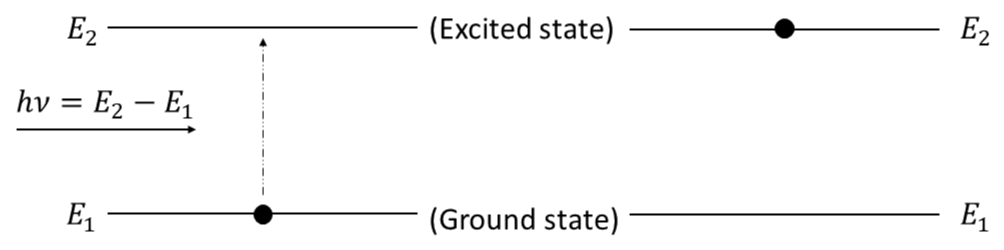
\includegraphics[width=0.5\textwidth]{indabs}
    \caption{Induced absorption}
    \label{indabs}
\end{figure}

An atom in the ground state with energy \(E_1\) absorbs an incident photon of energy \(h\nu\) and is excited to a higher energy state with energy \(E_2\) provided \(h\nu=E_2-E_1\). This process is known as induced absorption and is shown in \ref{indabs}. This type of interaction can be represented as
\[\text{atom}+\text{photon} \rightarrow \text{atom}^{\star}\]
where \(\text{atom}^{\star}\) is the excited state of the atom.

The excited atoms do not stay in the higher energy state for a longer time. It is the tendency of atoms in excited state to come to the lower energy state. Thus, the atoms in the excited state quickly return to the ground state by emitting a photon of energy \(h\nu\). The emission of photons takes place in two ways, namely spontaneous emission and stimulated emission.

\subsection{Spontaneous emission}
\label{subsec: Spontaneous emission}
\begin{figure}[h]
    \centering
    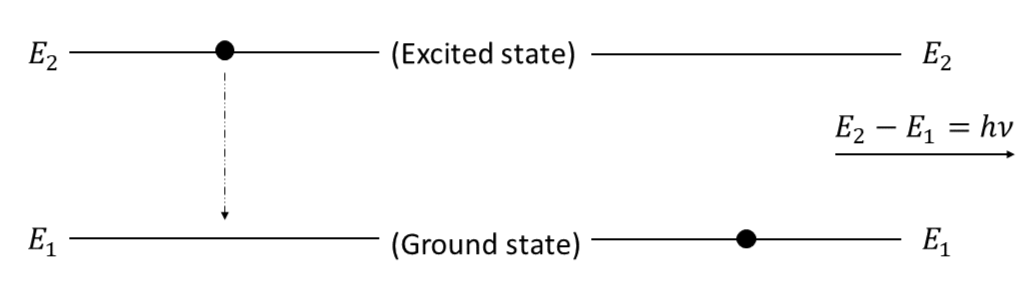
\includegraphics[width=0.5\textwidth]{spoemi}
    \caption{Spontaneous emission}
    \label{spoemi}
\end{figure}

The atom in the excited state \(E_2\) (higher energy state) stays there for around \(10^{-8}s\) and then returns to the ground \(E_1\) (lower energy state) by emitting a photon of energy \(h\nu\) such that \(E_2-E_1=h\nu\) without the influence of any external agency. Such an emission of light radiation which is not triggered by an external influence is called spontaneous emission. This process is shown in \ref{spoemi}. This type of interaction can be represented as
\[\text{atom}^{\star} \rightarrow \text{atom} + \text{photon}\]

It is a random and uncontrollable process. The photons emitted in this process travel in random directions.

\subsection{Stimulated emission}
\begin{figure}[h]
    \centering
    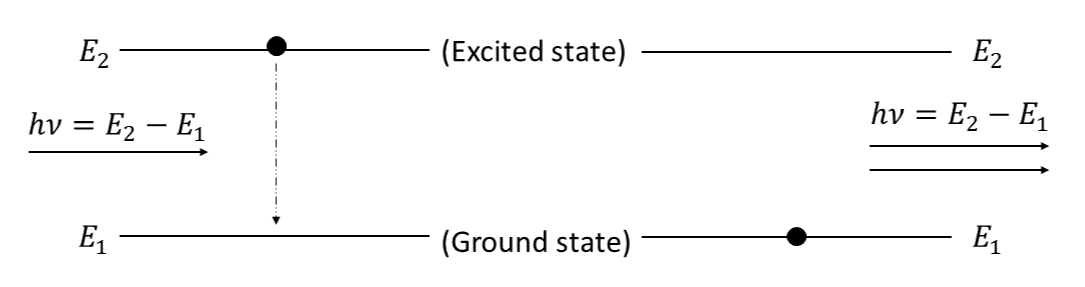
\includegraphics[width=0.5\textwidth]{stiemi}
    \caption{Stimulated emission}
    \label{stiemi}
\end{figure}

Einstein suggested that there must be another mechanism by which an atom in the excited state (\(E_2\)) can return to the ground state (\(E_1\)). He found that there is an interaction between the atom in excited state and a photon. During this interaction, the photon (of energy \(h\nu=E_2-E_1\)) triggers the excited atom to make a transition to the ground state. This transition produces a second (stimulated) photon which is similar to the triggering (stimulating) photon with respect to frequency, phase, and propagation direction. Such kind of forced emission of photons by the incident photons is called stimulated emission and is as shown in \ref{stiemi}. This type of interaction can be represented as
\[\text{atom}^{\star} + \text{photon} \rightarrow \text{atom} + \text{photon} + \text{photon}\]
This process plays a key role in the working of a laser.

\vspace{0.5cm}
In the next section, we use the term \(U_\nu\), the energy density. We can get \(U_\nu\) from \(U_\lambda\) after making appropriate substitutions. We have from Planck's law
\[U_\lambda d\lambda=\frac{8\pi hc}{\lambda^5}\left(\frac{1}{e^{\textstyle \frac{hc}{\lambda k_BT}}-1}\right)d\lambda\]

But we know that \(c=\nu\lambda\) or \(\displaystyle \lambda=\frac{c}{\nu}\).
Also, \(\displaystyle d\lambda = -\frac{c}{\nu^2}d\nu\) and \(U_\nu d\nu=-U_\lambda d\lambda\).

So after substitution, we get
\[U_\nu d\nu=\frac{8\pi h\nu^3}{c^3}\left(\frac{1}{e^{\textstyle \frac{h\nu}{k_BT}}-1}\right)\]

This is Planck's law in terms of frequency.

\section{Einstein's coefficients}
Consider an assembly of atoms with two energy states \(E_1\) and \(E_2\) at an absolute temperature \(T\). Let \(N_1\) be the number of atoms in state \(E_1\) and \(N_2\) be the number of atoms in state \(E_2\). Let light radiation of frequency \(\nu=(E_2-E_1)/h\) with energy density \(U_\nu\) be incident on this assembly of atoms. \(U_\nu\) is the number of photons incident on the system per unit area per unit time.

From statistical mechanics, for thermal equilibirum condition, there is a relation between an energy state \(E_i\) and the number of atoms \(N_i\) in that state. It is given as
\[N_i \propto e^{\frac{-E_i}{k_BT}}\]
For two energy states \(E_1\) and \(E_2\) such that \(E_2 > E_1\) and \((E_2-E_1)=h\nu\), we can write
\[\frac{N_1}{N_2}=\frac{e^{\frac{-E_1}{k_BT}}}{e^{\frac{-E_2}{k_BT}}}=e^{\frac{E_2-E_1}{k_BT}}=e^{\frac{h\nu}{k_BT}}\]

We notice here that since \((E_2-E_1)\) is positive, \(\frac{N_1}{N_2}>1\), which says that at thermal equilibrium condition, there are more number of atoms in the lower energy state than the higer energy state.

Now we write relations for the rate at which the three different process that we discussed above occur.

The rate of induced absorption is directly proportional to the number of atoms in the lower energy level \(N_1\) and the number of incident photons \(U_\nu\). So we have
\[\text{rate of induced absorption}\propto N_1 U_\nu\]
\[\text{rate of induced absorption}= B_{12} N_1 U_\nu\]
where \(B_{12}\) is the constant of proportionality called Einstein's coefficient for induced absorption.

The rate of spontaneous emission is directly proportional to the number of atoms in the higher energy level \(N_2\) only. This is because spontaneous emission occurs… well, spontaneously. \(U_\nu\) does not play any role in this interaction. So we have
\[\text{rate of spontaneous emission}\propto N_2\]
\[\text{rate of spontaneous emission}= A_{21} N_2\]
where \(A_{21}\) is the constant of proportionality called Einstein's coefficient for spontaneous emission.

The rate of stimulated emission is directly proportional to the number of atoms in the higher energy level \(N_2\) and the number of incident photons \(U_\nu\). So we have
\[\text{rate of stimulated emission}\propto N_2 U_\nu\]
\[\text{rate of stimulated emission}= B_{21} N_2 U_\nu\]
where \(B_{21}\) is the constant of proportionality called Einstein's coefficient for stimulated emission.

The Einstein's coefficients tell us about the probability of the respective processes occurring in the system.

At thermal equilibrium, the rate of all absorptions is equal to the rate of all emissions. So we have
\begin{multline*}
    \text{rate of induced absorption} = \text{rate of spontaneous emission }\\ + \text{ rate of stimulated emission}
\end{multline*}

Therefore, we have
\begin{align*}
    B_{12} N_1 U_\nu &= A_{21} N_2 + B_{21} N_2 U_\nu\\
    B_{12} N_1 U_\nu - B_{21} N_2 U_\nu &= A_{21} N_2\\
    (B_{12} N_1 - B_{21} N_2)U_\nu &= A_{21} N_2\\
    U_\nu &= \frac{A_{21} N_2}{B_{12} N_1 - B_{21} N_2}\\
    U_\nu &= \frac{A_{21} N_2}{B_{21} N_2} \left(\frac{1}{\frac{B_{12} N_1}{B_{21} N_2}-1}\right)
\end{align*}
But we know that
\[\frac{N_1}{N_2}=e^{\frac{h\nu}{k_BT}}\]

Thus, we have
\[U_\nu = \frac{A_{21}}{B_{21}} \left(\frac{1}{\frac{B_{12}}{B_{21}}e^{\frac{h\nu}{k_BT}}-1}\right)\]

Comparing this equation with the Planck's law (in terms of frequency), we see that
\[\frac{B_{12}}{B_{21}}=1 \text{ or } B_{12} = B_{21}\]
and
\[\frac{A_{21}}{B_{21}}=\frac{8\pi h\nu^3}{c^3}\]

Since \(B_{12} = B_{21}\), we can say that the probability of occurrence of induced absorption is equal to the probability of occurrence of stimulated emission. Further, we can drop the subscripts and simply write \(B_{12} = B_{21} = B\) and \(A_{21}=A\).

Therefore, the above equation can be written as
\[U_\nu = \frac{A}{B} \left(\frac{1}{e^{\frac{h\nu}{k_BT}}-1}\right)\]
This is the expression for energy density in terms of the Einstein's coefficients.

\subsubsection*{Consequences of the \(\frac{A}{B}\) relation}
We have the relation
\[\frac{A_{21}}{B_{21}}=\frac{8\pi h\nu^3}{c^3}\]
where \(\nu\) is the frequency of the incident photon, \(A_{21}\) and \(B_{21}\) are the probabilities for spontaneous emission and stimulated emission respectively.

Normally, for a system under thermal equilibrium, the probability for spontaneous emission is greater than that for stimulated emission. This is because by the time a stimulating photon can cause stimulated emission from an excited atom, the atom would already be de-excited and instead undergo spontaneous emission.

According to the above relation, the relative probability for spontaneous emission increases proportionally with the cube of frequency of the emitted photon. This means that it becomes more difficult to produce photons of higher frequencies from a laser. This is why we see blue and higher frequency lasers very rarely, because they are expensive to manufacture.

\section{Laser Action}

\subsection{Conditions for laser action}
Under normal conditions of thermal equilibrium in an atomic system, the number of atoms in the lower energy state will be more than that in the excited state (this is because atoms/molecules naturally tend to have lesser energy). In other words if \(N_1\) and \(N_2\) are the number densities of atoms in the lower and excited states respectively, then \(N_1 > N_2\). This can be shown as follows: if \(E_1\) and \(E_2\) are the energies of the atoms in the ground and excited states respectively, then according to the Boltzmann’s distribution function, we get
\[\frac{N_2}{N_1}=\frac{e^{-\frac{E_2}{k_BT}}}{e^{-\frac{E_1}{k_BT}}}=e^{-\frac{(E_2-E_1)}{k_BT}}\]
But we know that \((E_2-E_1)=h\nu\). So we get
\[\frac{N_2}{N_1}=e^{-\frac{h\nu}{k_BT}}\]

As \(E_2>E_1\), the RHS of the above equation is always less than unity, hence \(N_2 < N_1\).

But we know that lasers work under the principle of stimulated emission (it's in the name of LA\textbf{SE}R), and for this process, we need many atoms in the higher energy state. In other words, we need to make the system be in a situation where \(N_2 > N_1\). This situation, if attained, is called \underline{Population Inversion}.

The situation of population inversion can be achieved by exciting atoms from a lower energy state to a higher energy state by supplying energy from an external source. This act of supplying energy externally to attain population inversion is called \underline{Pumping}.

So after pumping, we have population inversion, i.e., \(N_2 > N_1\). But when an atom is excited to a higher energy state, it generally stays there for a very short amount of time, around \(10^{-8}\) seconds. This is such a short time that stimulated emission may not take place. So to realize stimulated emissions, we need the atoms in the excited states to stay there for a longer time. This is achieved by using elements which have a special kind of excited state called the \underline{Metastable state}. Atoms excited to these metastable states are found to stay there for around \(10^{-6} \text{ to } 10^{-3}\) seconds (which is 100 to, 100000 times longer than that for the regular excited states). If metastable states do not exist, then there is no population inversion, no stimulated emission, and hence no laser action.

\subsection{Requisites of a laser system}
\begin{itemize}
    \item \textbf{Active Medium:} It is the quantum system between whose energy levels the pumping and lasing action occurs.
    \item \textbf{Excitation Source:} To achieve population inversion, pumping is required. Pumping can be done in different ways, such as optical pumping, electrical pumping, and chemical pumping.
    \item \textbf{Laser Cavity:} The system containing the active medium between two mirrors of high reflectivity is called a \underline{laser cavity}. The mirrors reflect the photons produced due to stimulated emission to and fro through the active medium. Thus, the radiation inside the laser cavity builds up resulting in amplification of stimulated emission of radiation. Hence, the output of the system is a laser coherent light. Note that the length (\(L\)) of the cavity should be such that \(L=n\lambda /2\), where \(\lambda\) is the wavelength of the laser light, and \(n=1,2,3,\ldots\) (this is the condition for standing waves).
\end{itemize}


\end{document}
